\chapter{Atividades Realizadas}

\section{Protótipo das implementações do método}
A implementação do método foi toda feita utilizando orientação a objetos em C++, com excessão das funções específicas ao cálculo que possuem implementações, em CUDA, OpenCL e C++. Estas funções específicas ao cálculo consistem de operações básicas com vetores, aproximações para o campo vetorial e o método de Runge-Kutta em si. O código compartilhado entre as demais implementações vai desde as estruturas de dados até representações dos resultados em OpenGL.

O código pode ser encontrado em seu repositório Git em \newline\href{https://github.com/rafamanzo/runge-kutta}{https://github.com/rafamanzo/runge-kutta} é organizado basicamente em quatro pastas:
\begin{itemize}
  \item \textbf{core} contém as três implementações do método nas pastas \textit{c}, \textit{cuda} e \textit{opencl}; além das estruturas de dados que repensentam a entrada (\textit{dataset.cpp}) e a saída do método (\textit{fiber.cpp}).
  \item \textbf{example-factories} contém os scripts que geram arquivos de entrada para o protótipo de campos vetoriais sintéticos como exemplos;
  \item \textbf{includes} contém todos os cabeçalhos necessários, facilitando sua inclusão;
  \item \textbf{io} contém as classes que cuidam da entrada e saída do protótipo. A pasta \textit{gui} contém as abstrações utilizadas para a criação de uma interface gráfica com Glut e OpenGL. 
\end{itemize}

\newpage
As interações entre todas as classes que compõe podem ser vistas através do seguinte diagrama de classes:
\begin{figure}[!h]
  \begin{center}
    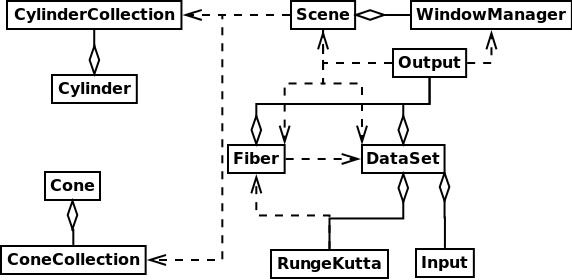
\includegraphics[width=120mm, height=60mm]{images/diagramadeclasse.png}
    \label{fig:}
    \caption{Diagrama de classes simplificado para o protótipo}
  \end{center}
\end{figure}

  \subsection{Estruturas compartilhadas em C++}
  A estrutura mais básica é a \textit{vector} contida em \textit{include/dataset.h}, consistindo de três \textit{doubles}, sua responsabilidade é representar tanto vetores quanto ponto no $\Re ^{3}$.
  
  \subsection{Método em C++}
  \subsection{Método em CUDA}
  \subsection{Método em OpenCL}
  \subsection{Geração de campos vetoriais sintéticos}
\section{Abstrações da VTK para uso de CUDA e OpenCL}
\section{Integração com o MedSquare através do VTK}
